\newcommand{\teasermanual}{
  \begin{subfigure}[b]{\linewidth}
    \centering
    \tikzsetnextfilename{teaser}
    {
      \def\firstrowimageheight{724px}
      \def\secondrowimagewidth{536px}
      \def\imageheight{2cm}
      \resizebox{\linewidth}{!}{
        \begin{tikzpicture}[
            >=stealth',
            overlay/.style={
                anchor=south west,
                draw=black,
                rectangle,
                line width=0.8pt,
                outer sep=0,
                inner sep=0,
              },
            font=\Huge
          ]
          \matrix[matrix of nodes, column sep=1pt, row sep=6em, ampersand replacement=\&, inner sep=0, outer sep=0, font=\Huge] (training) {
            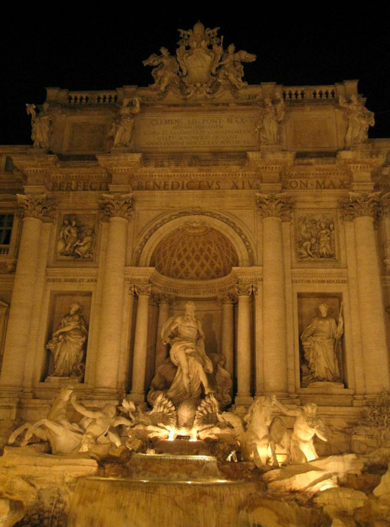
\includegraphics[width=\linewidth, trim={0 50 0 225}, clip]{\lumigaussassets/folder_for_kacper/teaser/training_and_rec.png} \&
            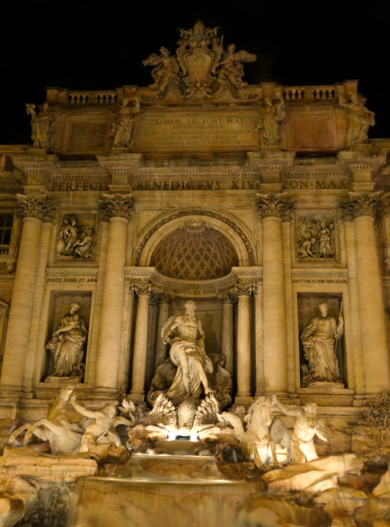
\includegraphics[width=\linewidth, trim={0 50 0 225}, clip]{\lumigaussassets/folder_for_kacper/teaser/rec.png} \&
            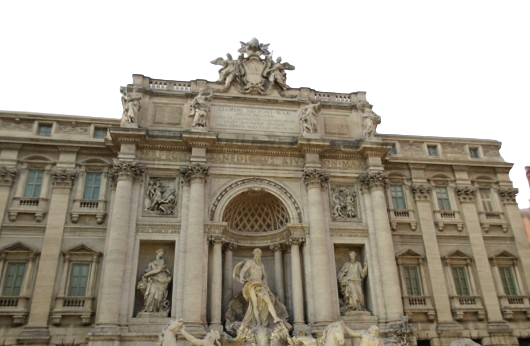
\includegraphics[width=\linewidth, trim={0 50 0 225}, clip]{\lumigaussassets/folder_for_kacper/teaser/albedo.png} \&
            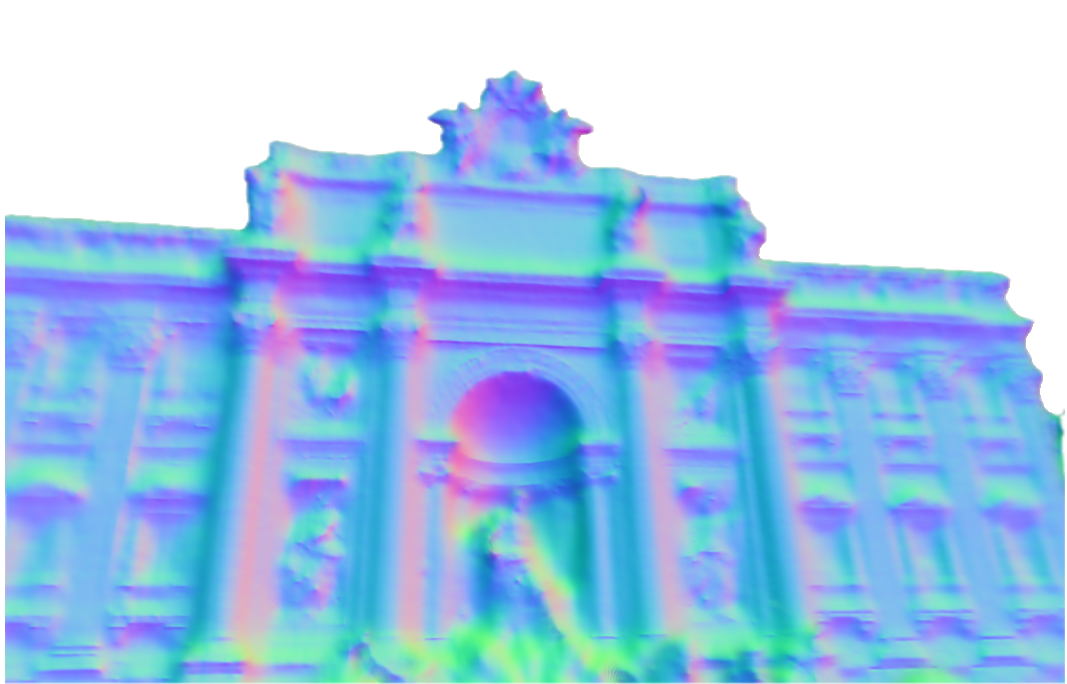
\includegraphics[width=\linewidth, trim={0 50 0 225}, clip]{\lumigaussassets/folder_for_kacper/teaser/normals.png} \\
            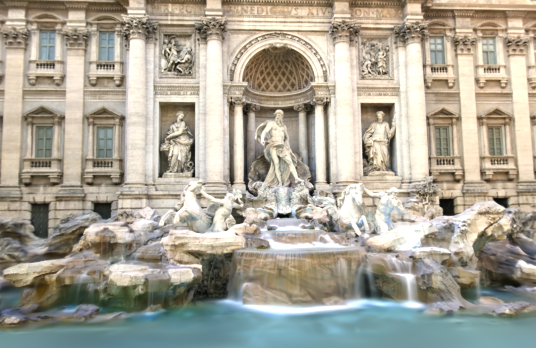
\includegraphics[width=\linewidth]{\lumigaussassets/folder_for_kacper/teaser/env_1_rec.png} \&
            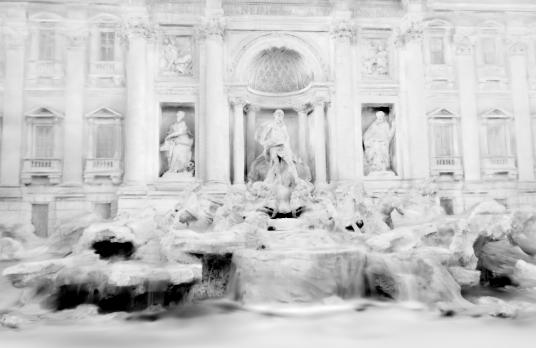
\includegraphics[width=\linewidth]{\lumigaussassets/folder_for_kacper/teaser/env_1_shadows.png} \&
            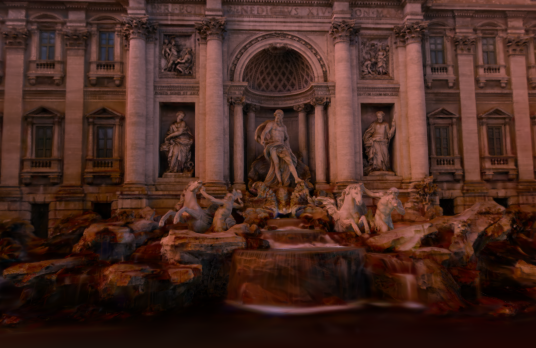
\includegraphics[width=\linewidth]{\lumigaussassets/folder_for_kacper/teaser/env_2_rec.png} \&
            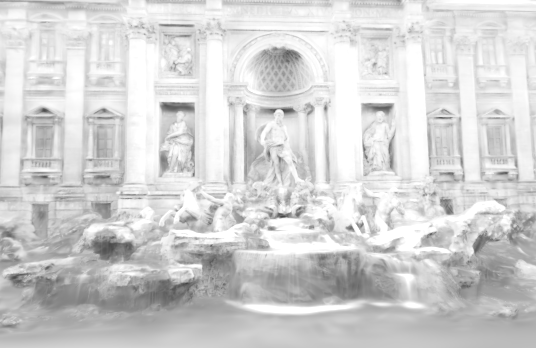
\includegraphics[width=\linewidth]{\lumigaussassets/folder_for_kacper/teaser/env_2_shadows.png}                                              \\
          };

          \node[above=1.6em of training-1-1.north, anchor=base,scale=1.3] {Training Image};
          \node[above=1.6em of training-1-2.north, anchor=base,scale=1.3] {Reconstruction};
          \node[above=1.6em of training-1-3.north, anchor=base,scale=1.3] {Predicted Albedo};
          \node[above=1.6em of training-1-4.north, anchor=base,scale=1.3] {Rendered Normals};

          \node[above=1.6em of training-2-1.north, anchor=base,scale=1.3] {Novel Light};
          \node[above=1.6em of training-2-2.north, anchor=base,scale=1.3] {Predicted Approximate Shadows};
          \node[above=1.6em of training-2-3.north, anchor=base,scale=1.3] {Novel Light};
          \node[above=1.6em of training-2-4.north, anchor=base,scale=1.3] {Predicted Approximate Shadows};

          \node[below right=5em and 1pt of training-2-1.north east, anchor=center]{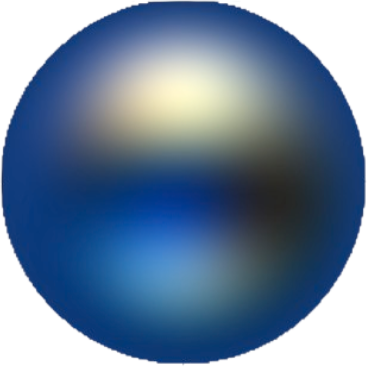
\includegraphics[width=4em]{\lumigaussassets/folder_for_kacper/teaser/env_1_map.png}};
          \node[below right=5em and 1pt of training-2-3.north east, anchor=center]{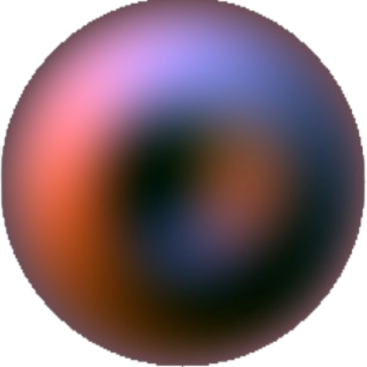
\includegraphics[width=4em]{\lumigaussassets/folder_for_kacper/teaser/env_2_map.png}};
        \end{tikzpicture}
      }
    }
  \end{subfigure}
}
\newcommand{\lumigaussteaserfigure}{
  \begin{figure}
    \centering
    \teasermanual
    \caption{
      \textbf{Teaser} --
      \lumigauss reconstructs environment maps and object surfaces from \textit{in-the-wild} images.
      Our model decouples the scene color and its normals (\textit{second and
      fourth column in the top row}).
      At inference, it can synthesize novel views (\textit{bottom row}) and
      realistic lighting (\textit{first and third columns in the bottom}) with
      high-fidelity shadows (\textit{second and fourth columns in the
      bottom}).
    }
    \label{fig:lumigauss-teaser}
  \end{figure}
}